\section{Fiber channel definition and capacity estimation}

\begin{figure}[htbp]
\centering
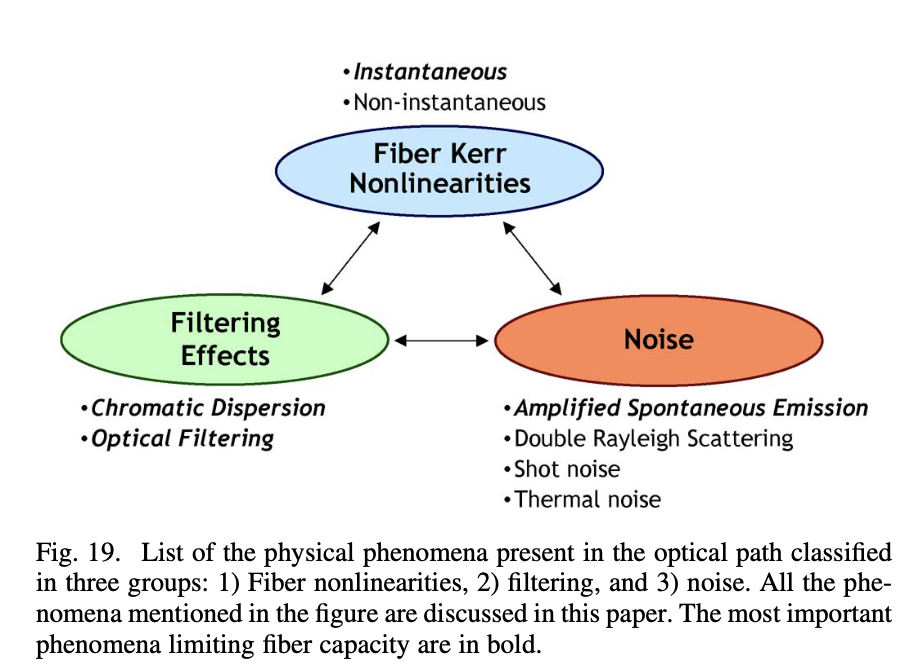
\includegraphics[width=0.5\linewidth]{img/noise.png}
\caption{channel noise term of optical fiber}
\label{noise of optical fiber}
\end{figure}

\begin{figure}[htbp]
\centering
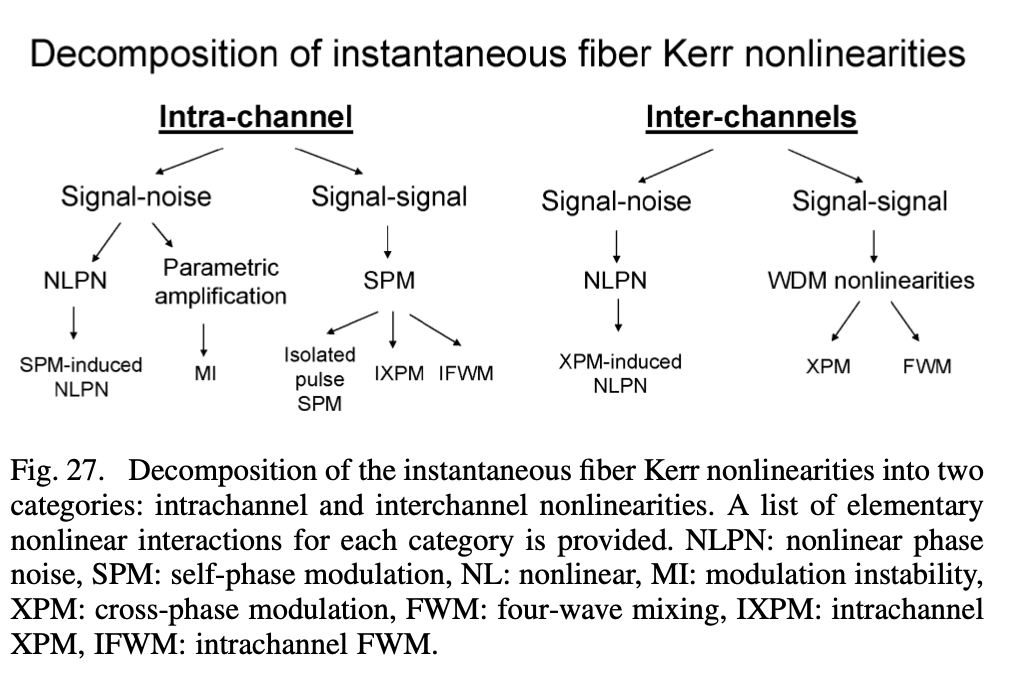
\includegraphics[width=0.5\linewidth]{img/nonlinearity.png}
\label{nopnlinearity}
\caption{Decomposition of fiber kerr nonlinearities}
\end{figure}

\begin{figure}
\centering
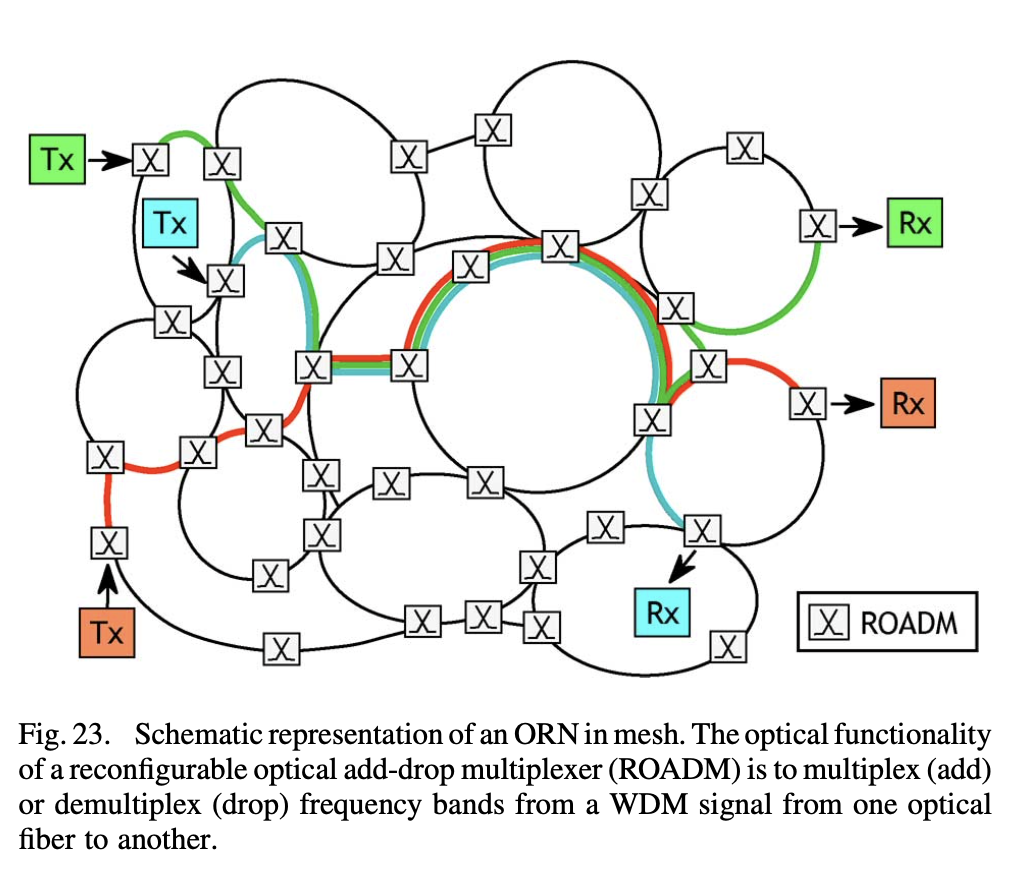
\includegraphics[width=0.5\linewidth]{img/ORN.png}
\caption{ORN}
\label{ORn}
\end{figure}

Stochastic generalized nonlinear Schrödinger equation:

\begin{equation}
\frac{\partial E}{\partial z}+\frac{i}{2} \beta_{2} \frac{\partial^{2} E}{\partial t^{2}}-i \gamma|E|^{2} E=i N(z, t)
\end{equation}

By statistical rotational invariance:

\begin{equation}
p\left(E_{\text {out }} \mid E_{\text {in }}\right)=p\left(E_{\text {out }} e^{i \Delta \phi} \mid E_{\text {in }} e^{i \Delta \phi}\right)
\end{equation}

next idea:
\begin{itemize}
\item Capacity with memory.
\item Capacity in discrete and continuous regime.
\item Example of calculating ring constellation.
\end{itemize}